% !TEX root = Master.tex

The study area is a private forest enterprise in Gartow (Niedersachsen) Germany. It measures around 5674.2 ha in total (see Table \ref{tab:sizes}) and is a relatively homogenous forest consisting mostly of pine trees.

\begin{table}[H]
\setlength\arrayrulewidth{1pt}  
\centering
\begin{tabular}{|c |c |c |c|}
\hline 
\rowcolor{Gray}
\textbf{Stratum} & \textbf{Location Class} & \textbf{Area [ha]} & \textbf{Relative Area} \\ 
\hline 
1 & 1 & 338.6 & 0.06 \\ 
\hline 
2 & 2 & 1546.9 & 0.27 \\ 
\hline 
3 & 3 & 2129.3 & 0.38 \\ 
\hline 
4 & 4 & 1550.5 & 0.27 \\ 
\hline 
G & 2 & 108.9 & 0.02 \\ 
\hline 
\rowcolor{SeaBlue}
Total & - & 5674.2 & 1 \\ 
\hline 
\end{tabular} 
\caption{Size of the different stratum and associated sampling grids. Stratum 2 and G have been merged to Location Class 2 which results in an identical sampling grid.}
\label{tab:sizes}
\end{table}

The forest itself is split into stratum to take site conditions, forest structure and thus natural variation of the areas into account (see Figure \ref{fig:Gartow Map}). The assessment of variation was based on a forest inventory conducted 2008
(see Table \ref{tab:Sample_Variation}).

\begin{table}[H]
\setlength\arrayrulewidth{1pt}  
\centering
\begin{adjustbox}{max width=\textwidth}
\begin{tabular}{|c |c |c |c |c |c |c |c|}
\hline 
\rowcolor{Gray}
\textbf{Stratum} & \textbf{Location Class} & \textbf{Area [ha]} & \textbf{Relative Area} & \textbf{Sample Size} & \textbf{Mean Volume / ha} & \textbf{Sample Variance} & \textbf{SE\%} \\ 
\hline 
1 & 1 & 338.6 & 0.06 & 159 & 180.19 & 104.24 & 5.67 \\ 
\hline 
2 & 2 & 1546.9 & 0.27 & 805 & 246.75 & 22.75 & 1.93 \\ 
\hline 
3 & 3 & 2129.3 & 0.38 & 542 & 195.41 & 13.15 & 1.86 \\ 
\hline 
4 & 4 & 1550.5 & 0.27 & 134 & 131.90 & 30.45 & 4.18 \\ 
\hline 
G & 2 & 108.9 & 0.02 & 55 & 271.26 & 734.08 & 9.99 \\ 
\hline 
\rowcolor{SeaBlue}
Total & - & 5674.2 & 1 & 1659 & 196.37 & 6.46 & 1.29 \\ 
\hline 
\end{tabular} 
\end{adjustbox}
\caption{Mean volume and sample variation estimates of the forest inventory 2008. Stratum 2 and 3 show little relative standard
error (SE\%), while stratum 1 inhibits more variation. Stratum G, which covers only 2\% of the total area has a typical high variation}
\label{tab:Sample_Variation}
\end{table}

Main sources of the variation in the growing stock can be assigned by the varieties in the tree species and the age distribution of the trees. Young and therefore small trees have a smaller diameter. If an area has been cultivated around the same timespan with identical species, the trees are expected to be centred on a certain diameter. On the other hand, a very diverse area in species and time will have naturally more variation (see Figure \ref{fig:barplots_Gartow})

\begin{figure}[H]
  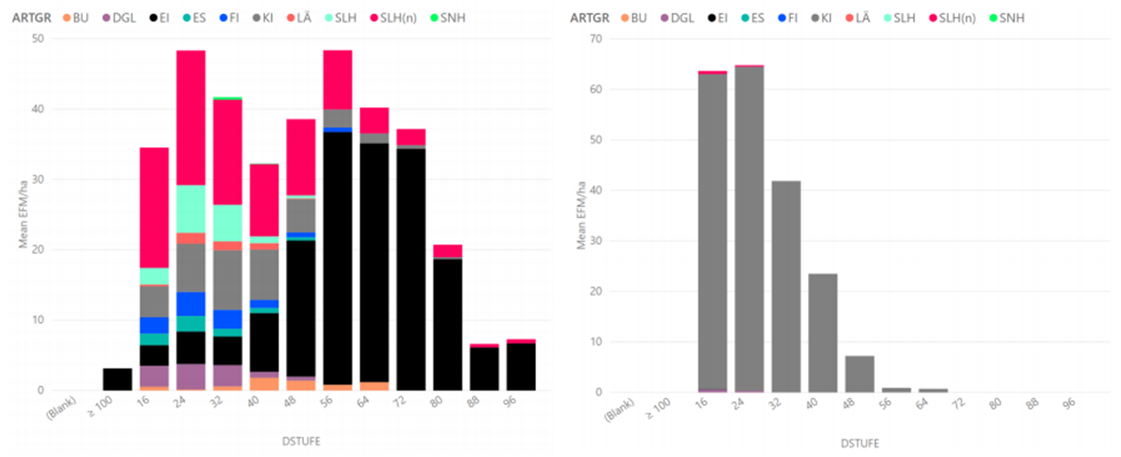
\includegraphics[width=\textwidth]{barplots_Gartow.png}
  \caption{The bar plots (left to right: stratum 1, stratum 4). The bars indicate the mean volume per ha for different diameter classes [1].}
  \label{fig:barplots_Gartow}
\end{figure}

Sampling activities are adjusting according to the inhibited variation of the stratum type (see Section \ref{Inventory Data}).

\begin{figure}[H]
  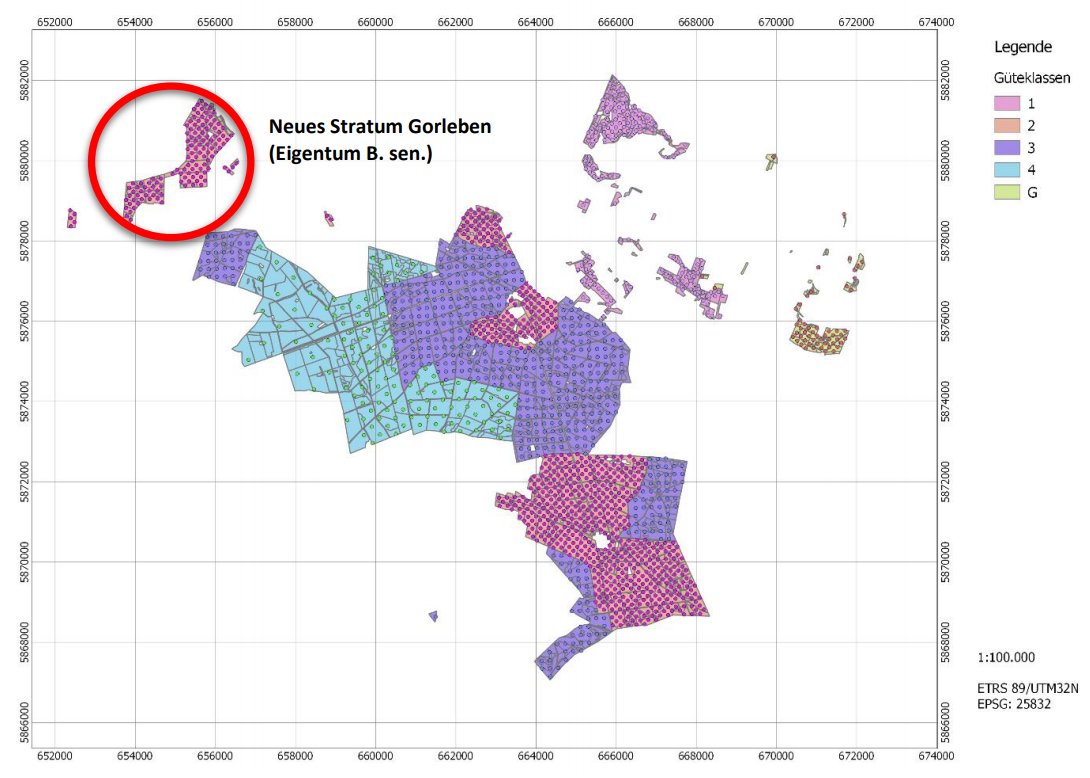
\includegraphics[width=\textwidth]{Gartow_map.png}
  \caption{The forest of Gartow is divided into stratums based on past observed variation and ownership and subdivided into compartments indicated by grey lines. Each point within a section indicate a sampling point [1].}
  \label{fig:Gartow Map}
\end{figure}

The stratum themselves are subdivided into compartments with the intention to create homogeneous sub regions (see Figure \ref{fig:Gartow Map}). The diameter distribution must be found for each of those compartments.
